\documentclass[12pt, a4paper, twoside]{article}

%% Preamble
\usepackage{umatfgspanish}
\usepackage{blindtext}
\usepackage[backend=biber]{biblatex}
\usepackage[all]{hypcap}
\bibliography{referencias}

\graphicspath{{images/}{../images/}}
\usepackage{subfiles} % Best loaded last in the preamble

\usepackage{listings}
\usepackage{color}
\definecolor{dkgreen}{rgb}{0,0.6,0}
\definecolor{gray}{rgb}{0.5,0.5,0.5}
\definecolor{mauve}{rgb}{0.58,0,0.82}

\lstdefinestyle{stylepython}{%
    frame=tb,
    language=python,
    aboveskip=3mm,
    belowskip=3mm,
    showstringspaces=false,
    columns=flexible,
    basicstyle={\small\ttfamily},
    numbers=none,
    numberstyle=\tiny\color{gray},
    keywordstyle=\color{blue},
    commentstyle=\color{dkgreen},
    stringstyle=\color{mauve},
    breaklines=true,
    breakatwhitespace=true,
    tabsize=3
}

\lstdefinestyle{swift}{%
    frame=tb,
    language=swift,
      aboveskip=3mm,
      belowskip=3mm,
      showstringspaces=false,
      columns=flexible,
      basicstyle={\small\ttfamily},
      numbers=none,
      numberstyle=\tiny\color{gray},
      keywordstyle=\color{blue},
      commentstyle=\color{dkgreen},
      stringstyle=\color{mauve},
      breaklines=true,
      breakatwhitespace=true,
      tabsize=1
}

\begin{document}

%% Cover

\includepdf[noautoscale=true, width=\paperwidth]{cover.pdf}

%% Title
\clearpage
\setcounter{page}{1}


\includepdf[noautoscale=true, width=\paperwidth]{title.pdf}

%\newpage

%% Abstract
\subfile{sections/abstract}

\newpage

\subfile{sections/resumen}

\tableofcontents

%% Sections
\section{Introducción}
\subfile{sections/introduccion}

\section{Bases del proyecto}
\subfile{sections/2-bases}

\section{API REST}
\subfile{sections/3-apirest}

\section{Extracción de características}
\subfile{sections/4-features}

\section{Modelo Deep Learning}
\subfile{sections/5-modeloML}

\section{ASL Interpreter}
\subfile{sections/6-interpreter}

\section{ Resultados y pruebas}
\subfile{sections/7-resultados}

\section{Conclusiones y Líneas Futuras}
\subfile{sections/conclusiones}

%% Bibliography
\printbibliography[title={Bibliografía}, heading=bibintoc]

\newpage

%% Apendices
\begin{umaappendices}
  \section{Jupyter Notebook}\label{notebook}
  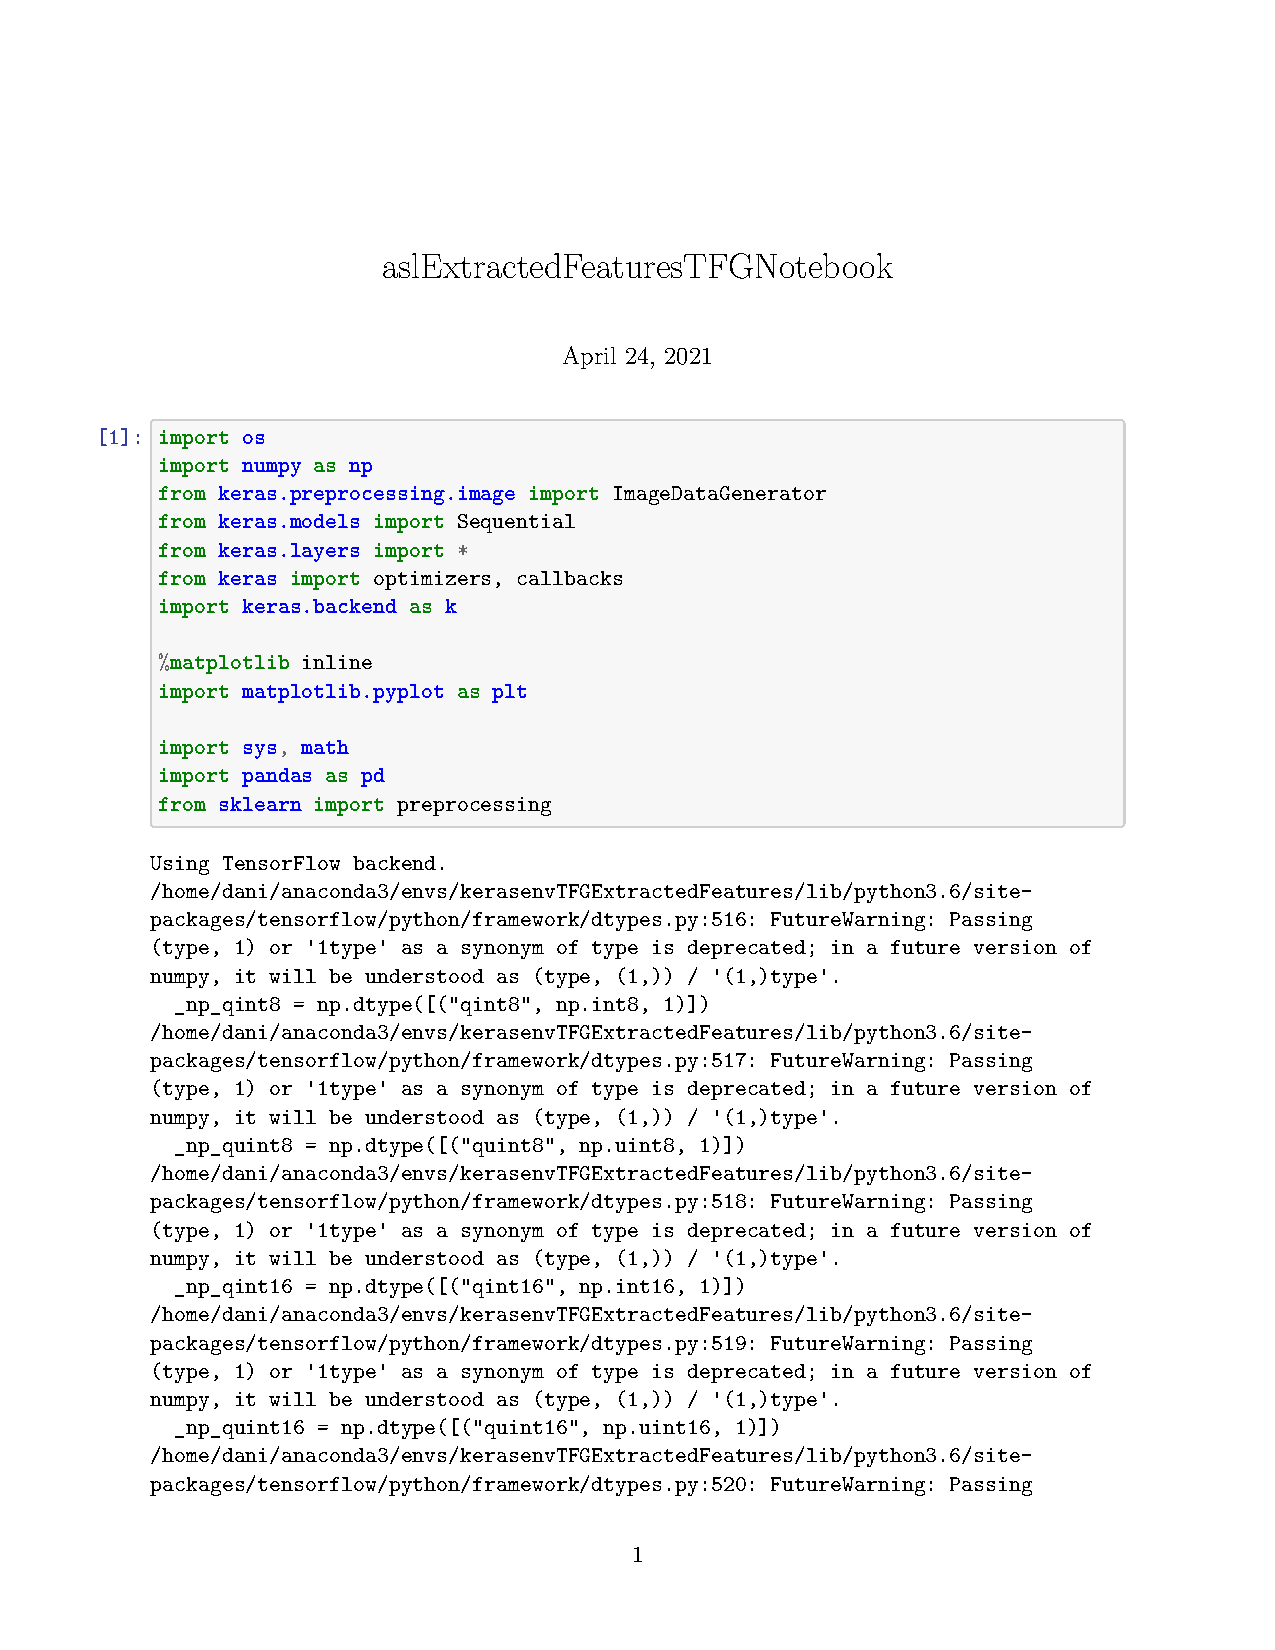
\includepdf[pages=-]{notebook/notebook.pdf}
  

\end{umaappendices}

%% Back Cover

\includepdf[noautoscale=true, width=\paperwidth]{backcover.pdf}
\end{document}
